\let\negmedspace\undefined
\let\negthickspace\undefined
\documentclass[journal]{IEEEtran}
\usepackage[a5paper, margin=10mm, onecolumn]{geometry}
\usepackage{lmodern} % Ensure lmodern is loaded for pdflatex
\usepackage{tfrupee} % Include tfrupee package

\setlength{\headheight}{1cm} % Set the height of the header box
\setlength{\headsep}{0mm}     % Set the distance between the header box and the top of the text

\usepackage{gvv-book}
\usepackage{gvv}
\usepackage{cite}
\usepackage{amsmath,amssymb,amsfonts,amsthm}
\usepackage{algorithmic}
\usepackage{graphicx}
\usepackage{textcomp}
\usepackage{xcolor}
\usepackage{txfonts}
\usepackage{listings}
\usepackage{enumitem}
\usepackage{mathtools}
\usepackage{gensymb}
\usepackage{comment}
\usepackage[breaklinks=true]{hyperref}
\usepackage{tkz-euclide} 
\usepackage{listings}
\usepackage{gvv}                                        
\def\inputGnumericTable{}                                 
\usepackage[latin1]{inputenc}                                
\usepackage{color}                                            
\usepackage{array}                                            
\usepackage{longtable}                                       
\usepackage{calc}                                             
\usepackage{multirow}                                         
\usepackage{hhline}                                           
\usepackage{ifthen}                                           
\usepackage{lscape}
\begin{document}

\bibliographystyle{IEEEtran}
\vspace{3cm}

\title{4-4.2-1}
\author{EE24BTECH11005 - Arjun Pavanje}
% \maketitle
% \newpage
% \bigskip
{\let\newpage\relax\maketitle}
Question:\\
Find the direction and normal vectors of the given line $2x+3y=9$
\begin{table}[h!]    
  \centering
  \begin{tabular}[12pt]{ |c| c|}
    \hline
    \textbf{Variable} & \textbf{Description}\\ 
    \hline
	$\vec{a}$ & $BC$ line\\
   \hline
	$\vec{b}$ & $AC$ line\\
   \hline
	$\vec{c}$ & $AB$ line, $5cm$ length\\
   \hline
	$\vec{K}$ & $a+b=5cm$\\
	\hline
	$\vec{\angle{A}}$ & $\angle{BAC}=45{\degree}$\\
	\hline

    \end{tabular}

  \caption{Variables Used}
  \label{tab1-1.9-6}
\end{table}\\
\solution
The equation of the line is given by,
\begin{align}
	y&=mx+c\\
	\vec{x}&=\myvec{0\\c}+ x \myvec{1\\m}\\
	\vec{x}&=\vec{h}+k\vec{m}
\end{align}
here, $\vec{m}=\myvec{1\\m}$ where $\vec{m}$ is direction vector\\
given line can be written as\\
$$\vec{x}=\myvec{0\\3}+k\myvec{3\\-2}$$
$$\vec{m}=\myvec{3\\-2}$$
equation of line in terms of normal vector $\vec{n}$ is,
\begin{align}
\vec{n}^T\vec{x}=c\\
	\vec{n}=\myvec{-m\\1}
\end{align}
Here, $$\vec{n}=\myvec{2\\3}$$
Direction vector: $\vec{m}=\myvec{3\\-2}$\\
Normal Vector: $\vec{n}=\myvec{2\\3}$
\begin{figure}[h!]
   \centering
   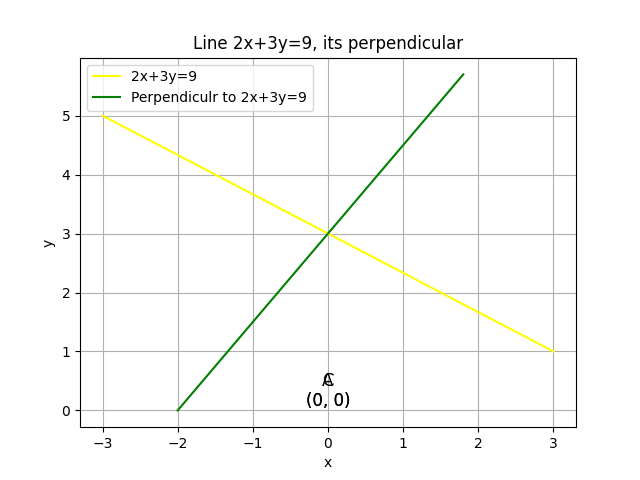
\includegraphics[width = 1\linewidth]{figs/fig.png}
   \caption{Plot of the line}
   \label{stemplot}
\end{figure}
\end{document}
